%!TEX root = thesis.tex
\chapter{Tensor Network Theory}
In tensor network theory, we are used to represent tensors graphically instead of complicated equations, because \textit{tensor diagrams} can map to quantum states and geometric lattices explicitly. Base on its clearly representation, we can implement tensor network algorithms simply. This section begins from a fundamental question: How to draw a tensor network diagrams?

\section{Representation of tensors in tensor Networks}
\label{notations}
In mathematical concept, a tensor is considered as a multi-dimensional array of scalers. The arrangement of the elements in a tensor is dependent to its \textit{indices} and the \textit{rank} of tensor is equivalent to the number of indices. Thus, a rank-0 tensor is a scaler $(T)$, a rank-1 tensor is a vector $(T_{i})$, a rank-2 tensor is a matrix $(T_{ij})$ and so on. 

Graphically, we usually use a node and few bonds to represent a tensor. Some specified examples are shown in figure \ref{fig211}, the number of bond is equal to the rank of tensor, which means that tensors without bonds, with a single bond, with two bonds and with three bonds can map to scalers, vectors, matrices and rank-3 tensor.

	\begin{figure}[ht]
	\centering
	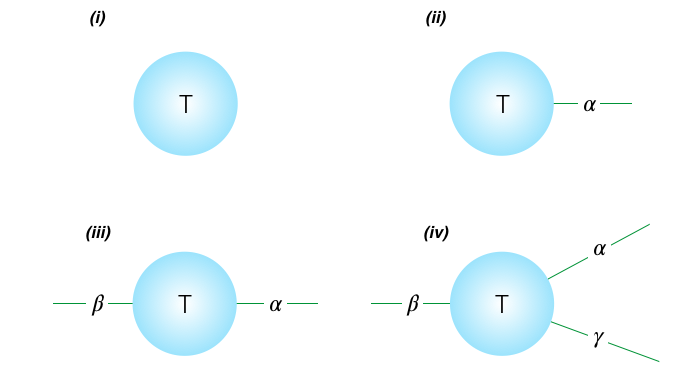
\includegraphics[width=0.75\textwidth]{figures/fig211.png}
	\caption[The reprecentation of commen tensors.]{Usually we use a note and few bonds to compose a tensor and the numbers of bond depend on the rank of tensor. (i) A tensor without bonds is a scaler $T$, (ii) A tensor with one bond is a vector $T_{\alpha}$, (iii) A tensor with two bonds is a Matrix $T_{\alpha \beta}$, (iv) A tensor with three bonds is a rank-3 tensor $T_{\alpha \beta \gamma}$.}
	\label{fig211}
	\end{figure}

	Then, we should determine the dimension of tensors. Explicitly, the dimension of rank=0 (scaler) is equal to one. However, the dimension of tensors higher than rank-0 depend on the bond dimensions. For instance, in Fig.\ref{fig211}(iv), it's a rank-3 tensor and the dimensions of the indices are $\chi_{\alpha}$, $\chi_{\beta}$, $\chi_{\gamma}$ and T contains $\chi_{\alpha}$$\chi_{\beta}$$\chi_{\gamma}$ components.

\section{Tensor operations and tensor network diagrams} % (fold)
\label{operation}
Basically we can't calculate an fold tensors directly. So the first step, we should unfold tensors. On the other words, we must make their rank lower than 3 before operating. In order to explaining clearly, I give bond two different types, incoming (BD\_IN) and outgoing (BD\_OUT) bond, which is on node's left and right. Further explanation, BD\_IN and BD\_OUT can be imagined as rows and columns of a matrix. For instance, if the indices of $T_{\alpha \beta \gamma}$ ordered like Fig\ref{fig221}(i), it means that $T_{\alpha \beta \gamma}$ is a matrix $T_{\chi_{\beta}\chi_{\gamma},\chi_{\alpha}}$. Similarity, If it's like Fig\ref{fig221}(ii), it means that $T_{\alpha \beta \gamma}$ is a matrix $T_{\chi_{\beta},\chi_{\alpha}\chi_{\gamma}}$.

	\begin{figure}[ht]
	\centering
	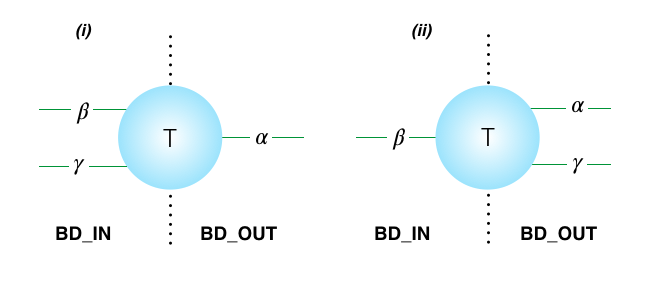
\includegraphics[width=0.75\textwidth]{figures/fig221.png}
	\caption[Representaion of unfold tensors.]{(i) Unfold a tensor to a matrix $T_{\chi_{\beta}\chi_{\gamma},\chi_{\alpha}}$, (ii) Unfold a tensor to a matrix $T_{\chi_{\beta},\chi_{\alpha}\chi_{\gamma}}$.}
	\label{fig221}
	\end{figure}

\subsection{Shape}

\subsection{Permutation}

\section{Reducing Computational Complexity} % (fold)
\label{sub:reduce}

Make simulation possible and improve the accuracy and efficiency.
